\documentclass[14pt]{extarticle}

\usepackage{fontspec}
\setmainfont{Times New Roman}

% размер полей
\usepackage{geometry}
\geometry{a4paper, top=2cm, bottom=2cm, right=1.5cm, left=3cm}

 %debugging
%\usepackage{showframe}

% полуторный интервал
\usepackage{setspace}
\onehalfspacing

% абзацный отступ
\setlength{\parindent}{1.25cm}

% выравнивание текста по ширине
\sloppy

% списки
\usepackage{calc} % арифметические операции с величинами
\usepackage{enumitem}
\setlist{
    nosep,
    leftmargin=0pt,
    itemindent=\parindent + \labelwidth - \labelsep,
}

% подписи к рисункам и таблицам
\usepackage{caption}
\renewcommand{\figurename}{Рисунок}
\renewcommand{\tablename}{Таблица}
\DeclareCaptionFormat{custom}
{
    \textit{#1#2#3}
}
\DeclareCaptionLabelSeparator{custom}{. }
\captionsetup{
    % хз какой это размер - 12 или нет, но выглядит меньше 14
    font=small,
    format=custom,
    labelsep=custom,
}

% картинки
\usepackage{graphicx}

% колонтитулы
\usepackage{fancyhdr}

% картинки и таблицы находятся именно в том месте текста где помещены (атрибут H)
\usepackage{float}

% таблицы
\usepackage{tabularray}

\graphicspath{ {7.2.1/models/} }
\begin{document}
\pagestyle{fancy}
\fancyhead{}
% disable header
\renewcommand{\headrulewidth}{0pt}
\fancyfoot[L]{Дубровских гр 221-361}
\fancyfoot[C]{ЛР 7.2.1}
\fancyfoot[R]{Продажа автотранспорта}
\singlespacing

\newpage
\begin{center}
    Министерство науки и высшего образования Российской Федерации
    Федеральное государственное автономное образовательное учреждение

    высшего образования

    \guillemotleft МОСКОВСКИЙ ПОЛИТЕХНИЧЕСКИЙ УНИВЕРСИТЕТ\guillemotright

    (МОСКОВСКИЙ ПОЛИТЕХ)
\end{center}
\noindent
\bigbreak
\bigbreak
\bigbreak
\bigbreak
\begin{center}
    ЛАБОРАТОРНАЯ РАБОТА 7.2.1

    По курсу Проектирования пользовательских интерфейсов в веб

    \textbf{Выбор и построение модульных сеток сайта и мобильного приложения, создание макетов для нескольких устройств}
    \bigbreak
    \bigbreak
    \bigbreak
    \bigbreak
    ТЕМА

    \guillemotleft\textbf{САЙТ ДЛЯ ПРОДАЖИ И ПОИСКА АВТОМОБИЛЕЙ}\guillemotright
\end{center}
\noindent
\bigbreak
\bigbreak
\bigbreak
\bigbreak
\bigbreak
\bigbreak
\bigbreak
\bigbreak
\bigbreak
\bigbreak
\hfill Выполнил

\hfill Дубровских Никита Евгеньевич

\hfill Группа 221-361
\bigbreak
\bigbreak
\bigbreak
\hfill Проверил

\hfill Натур ВВ
\vfill
\begin{center}
    Москва, 2024
\end{center}
\newpage
\onehalfspacing


\begin{center}
    \textbf{Лабораторная работа 7.2.1}

    \textbf{Выбор и построение модульных сеток сайта и мобильного приложения, создание макетов для нескольких устройств}
\end{center}

\textbf{Цель работы:} создать модульную сетку и расположить контента интерфейса
\bigskip

\textbf{Задачи:}

\begin{enumerate}
    \item Подобрать модульную сетку для веб-страниц.
    \item Изучить адаптивную и респонсивную верстку.
    \item Создать адаптивный макет для нескольких устройств
\end{enumerate}
\bigskip

\textbf{Основные термины}

\begin{itemize}
    \item Модульная сетка — это система невидимых линий, на которой располагаются элементы дизайна для создания структурированной, логичной и удобной компоновки элементов. Модульные сетки помогают упорядочить элементы, улучшая восприятие и навигацию.
    \item Адаптивный дизайн — подход к веб-дизайну, при котором создаются несколько фиксированных макетов для различных устройств. Выбор конкретного макета зависит от экрана пользователя. Это дает возможность оптимизировать работу сайта или приложения для конкретного устройства.
    \item Респонсивный (отзывчивый) дизайн — дизайн, который подстраивается под размеры экрана с помощью гибкой сетки и CSS медиа-запросов. Элементы изменяются автоматически, позволяя интерфейсу быть адаптивным к различным разрешениям.
    \item Колонки — основные вертикальные сегменты сетки, определяющие структуру. Колонки можно разделить на несколько частей (например, 12 колонок), что позволяет гибко использовать пространство.
    \item Межколоночный интервал — пространство между колонками. Оно играет роль микро-пробела, добавляя «воздуха» в макет. Размер интервала влияет на визуальное восприятие интерфейса.
    \item Поля (уши) — края сетки, которые остаются пустыми для создания визуального баланса. Рекомендуется использовать фиксированное поле слева и справа для аккуратного оформления макета.
    \item Пропорциональные зависимости — балансирование визуальных элементов через соблюдение пропорций, что позволяет создавать гармоничный интерфейс и выделять важные части компоновки.
\end{itemize}
\bigskip

\textbf{Выбор модульной сетки}

Была выбрана 12-колоночатая сеткa для макета, так как онa обеспечивает гибкость и адаптивность, позволяя легко управлять контентом для разных экранов и устройств. Вот основные причины выбора:
\begin{itemize}
    \item 12 колонок позволяют делить макет на 2, 3, 4, 6 частей, что даёт возможность создания разнообразных компоновок контента;
    \item такая сетка легко адаптируется под различные разрешения, обеспечивая плавное изменение ширины колонок, что делает её удобной для адаптивного дизайна;
    \item 12-колоночная сетка — это стандарт в большинстве CSS-фреймворков (например, Bootstrap), что упрощает разработку и делает дизайн более предсказуемым и удобным для пользователей;
    \item разделение на 12 колонок позволяет создать визуально сбалансированный макет, что облегчает восприятие и навигацию для пользователей.

\textbf{Макеты по сетке}
\bigskip

\noindent
\begin{minipage}{\linewidth}
    \fbox{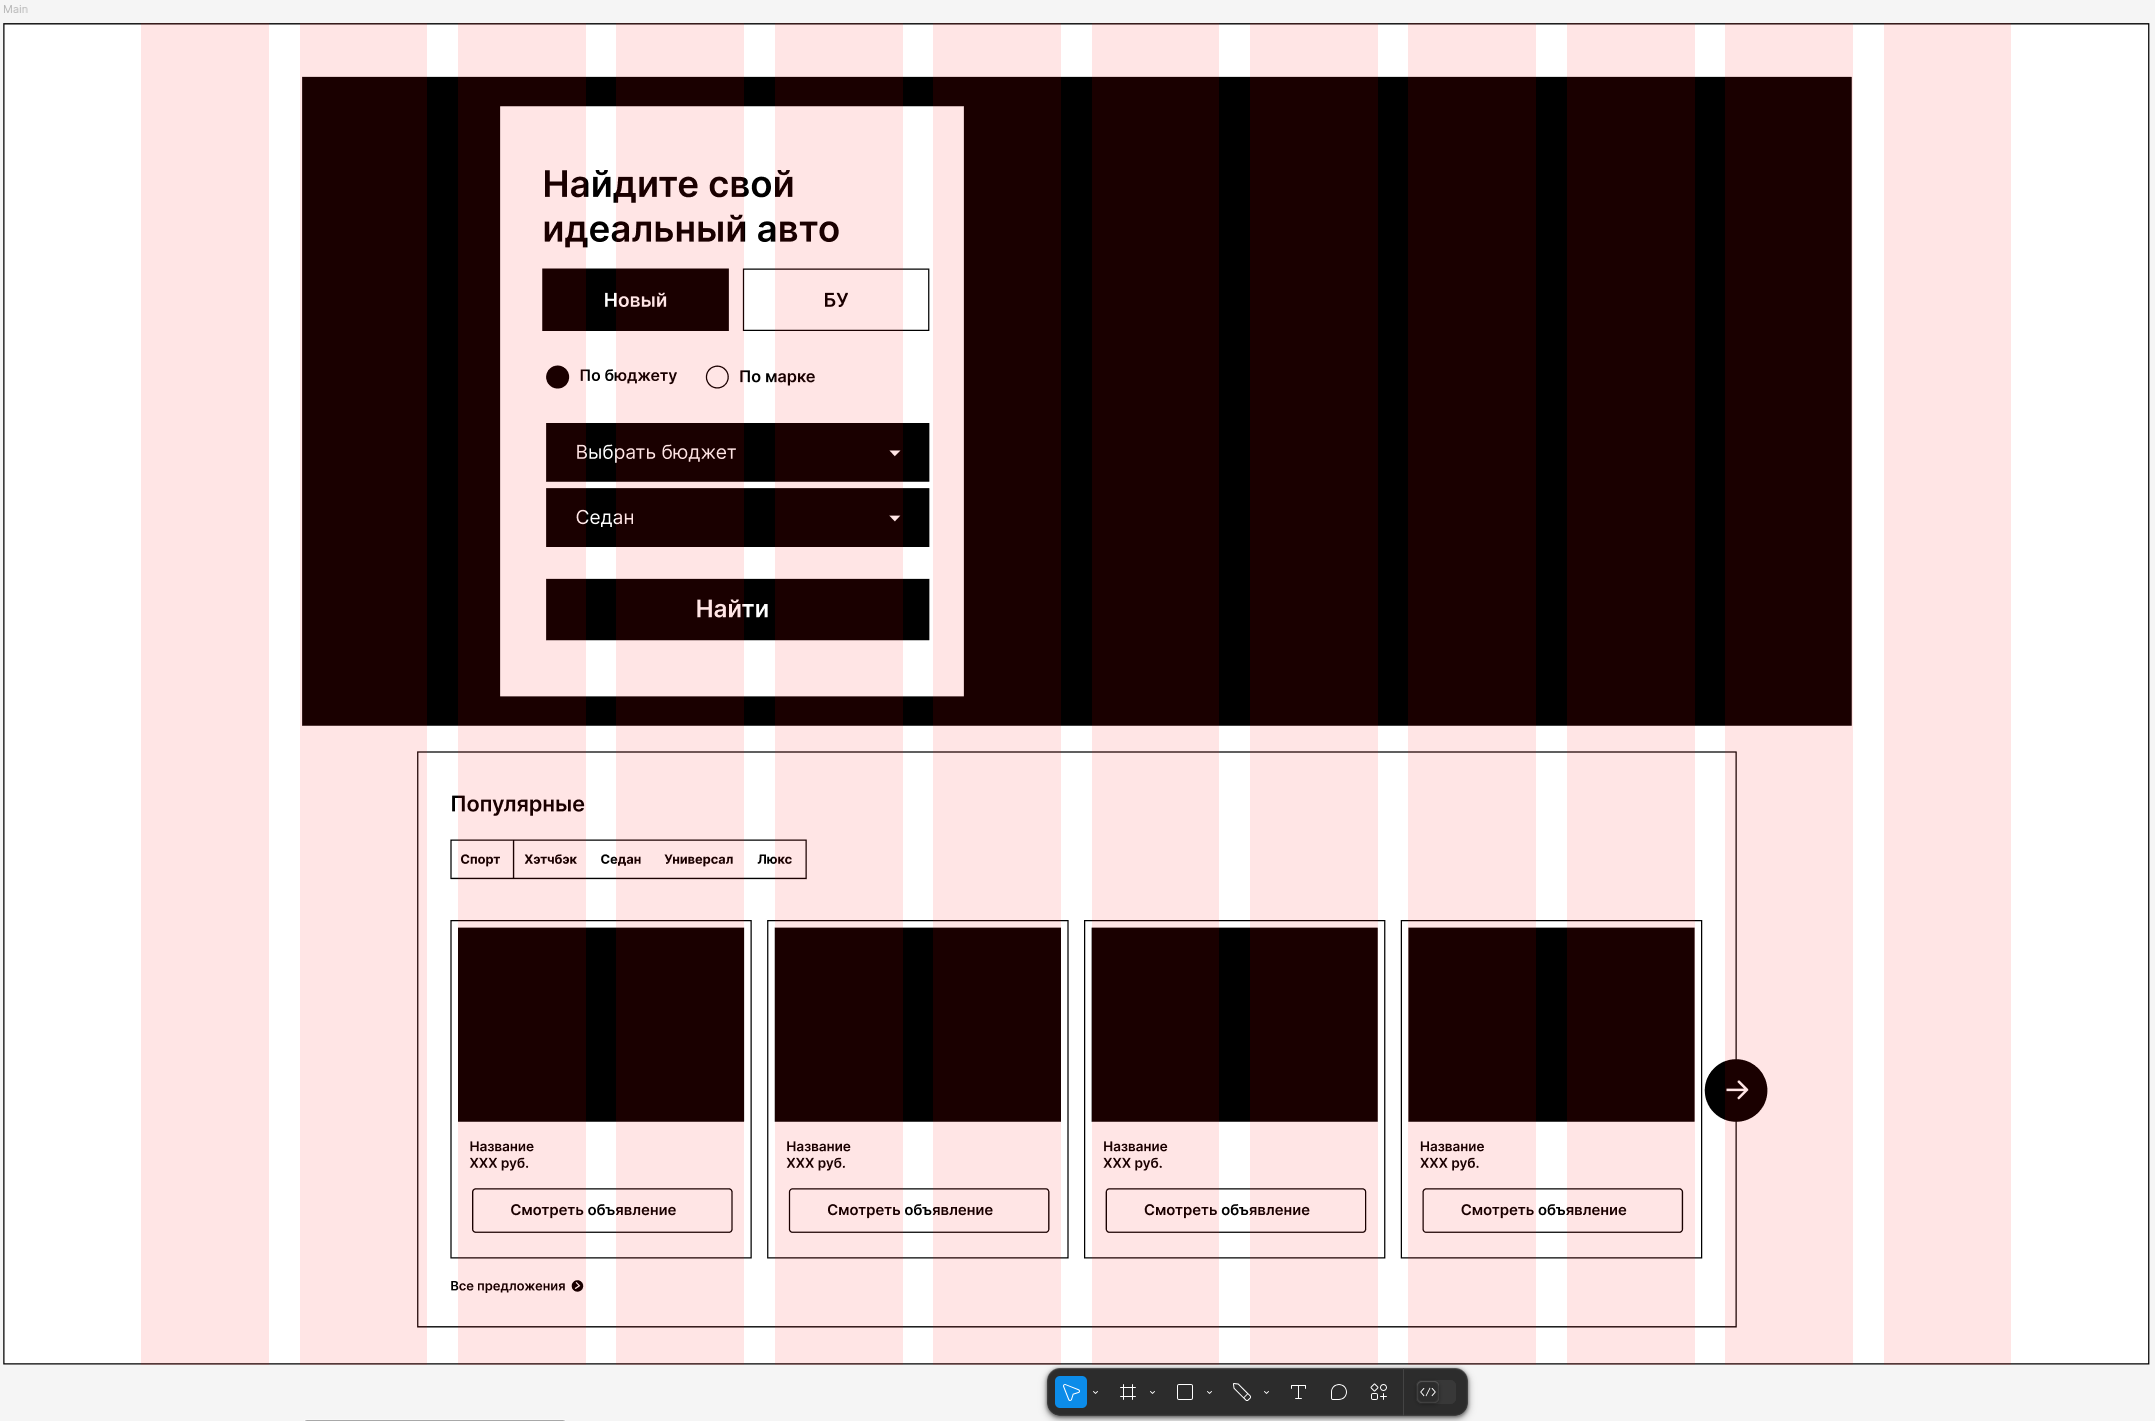
\includegraphics[width=\linewidth]{main}}
    \captionof{figure}{Главная страница}
\end{minipage}
\bigskip

\noindent
\begin{minipage}{\linewidth}
    \fbox{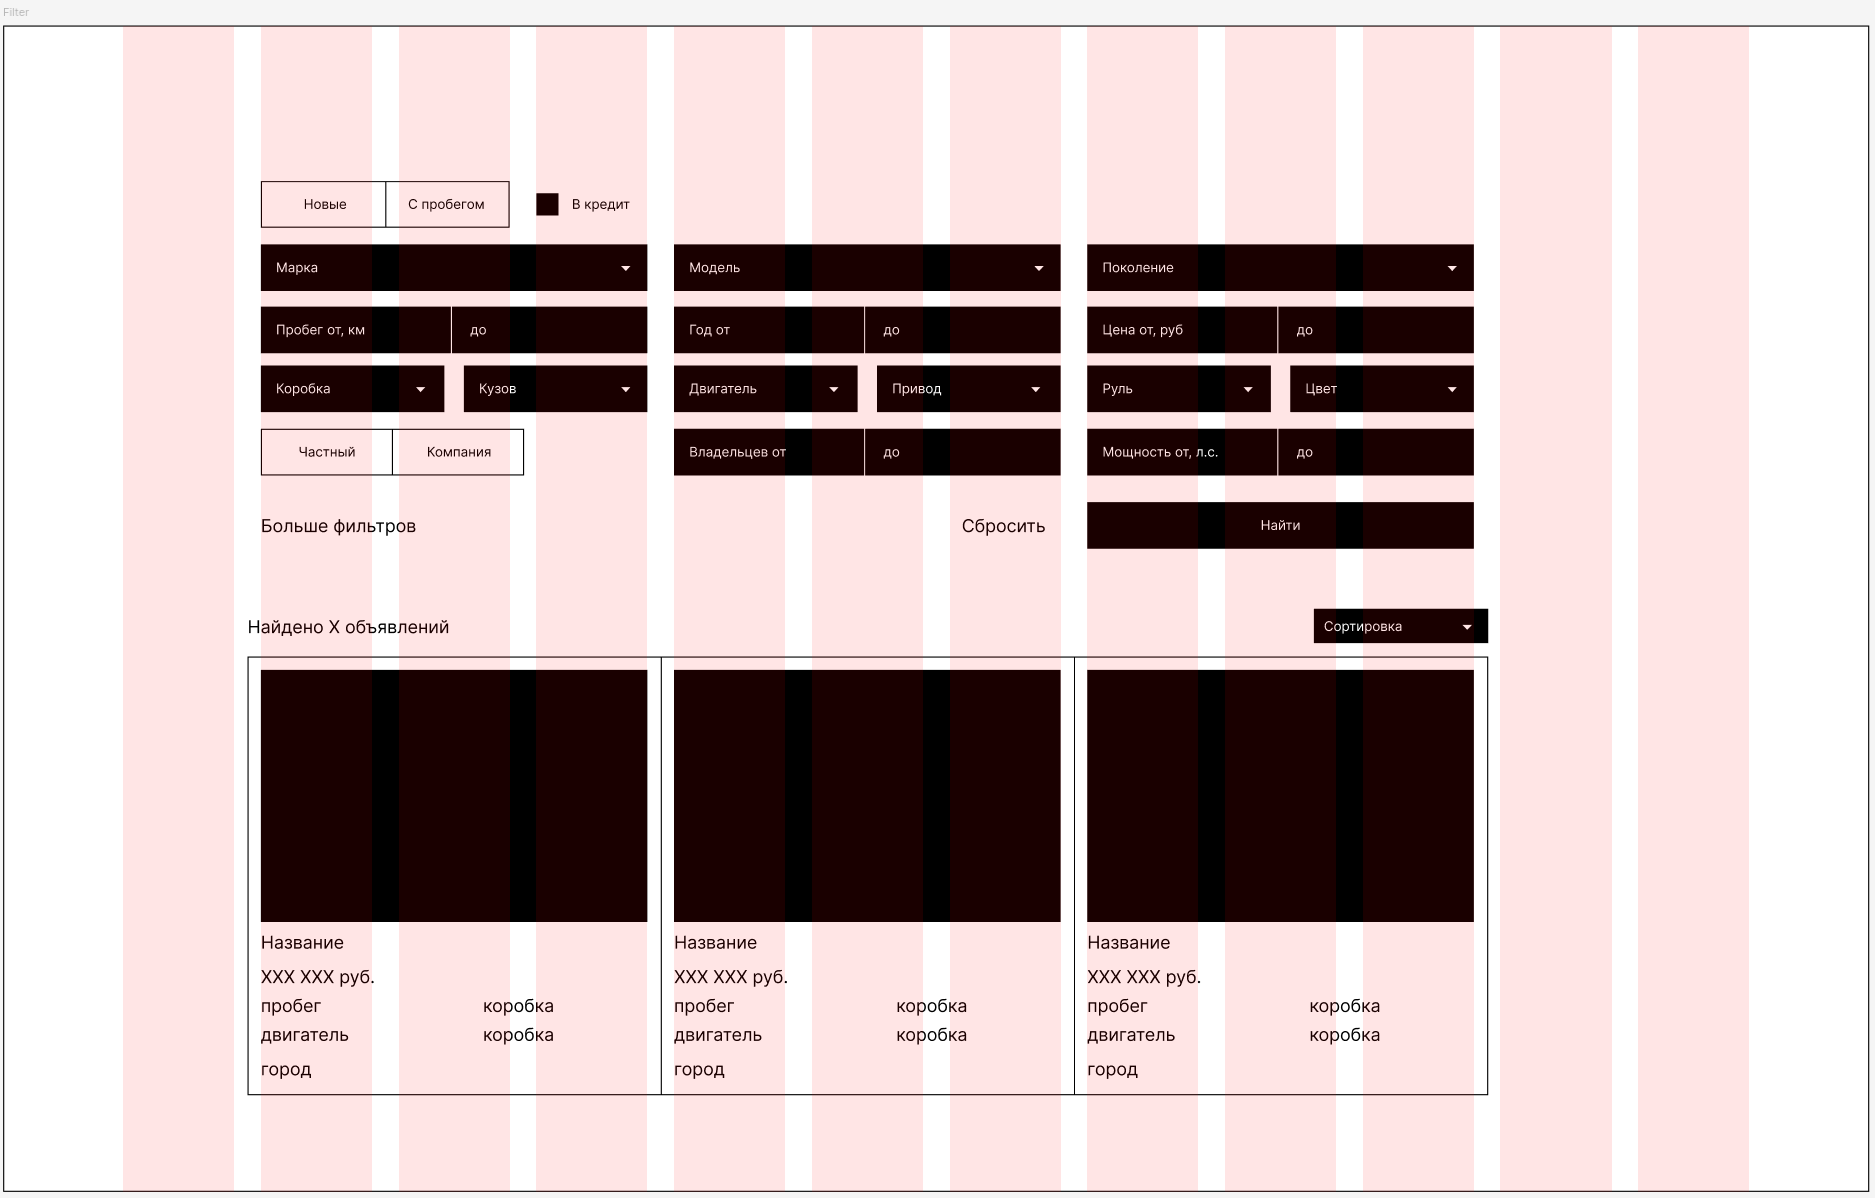
\includegraphics[width=\linewidth]{filter}}
    \captionof{figure}{Фильтры}
\end{minipage}
\bigskip

\noindent
\begin{minipage}{\linewidth}
    \fbox{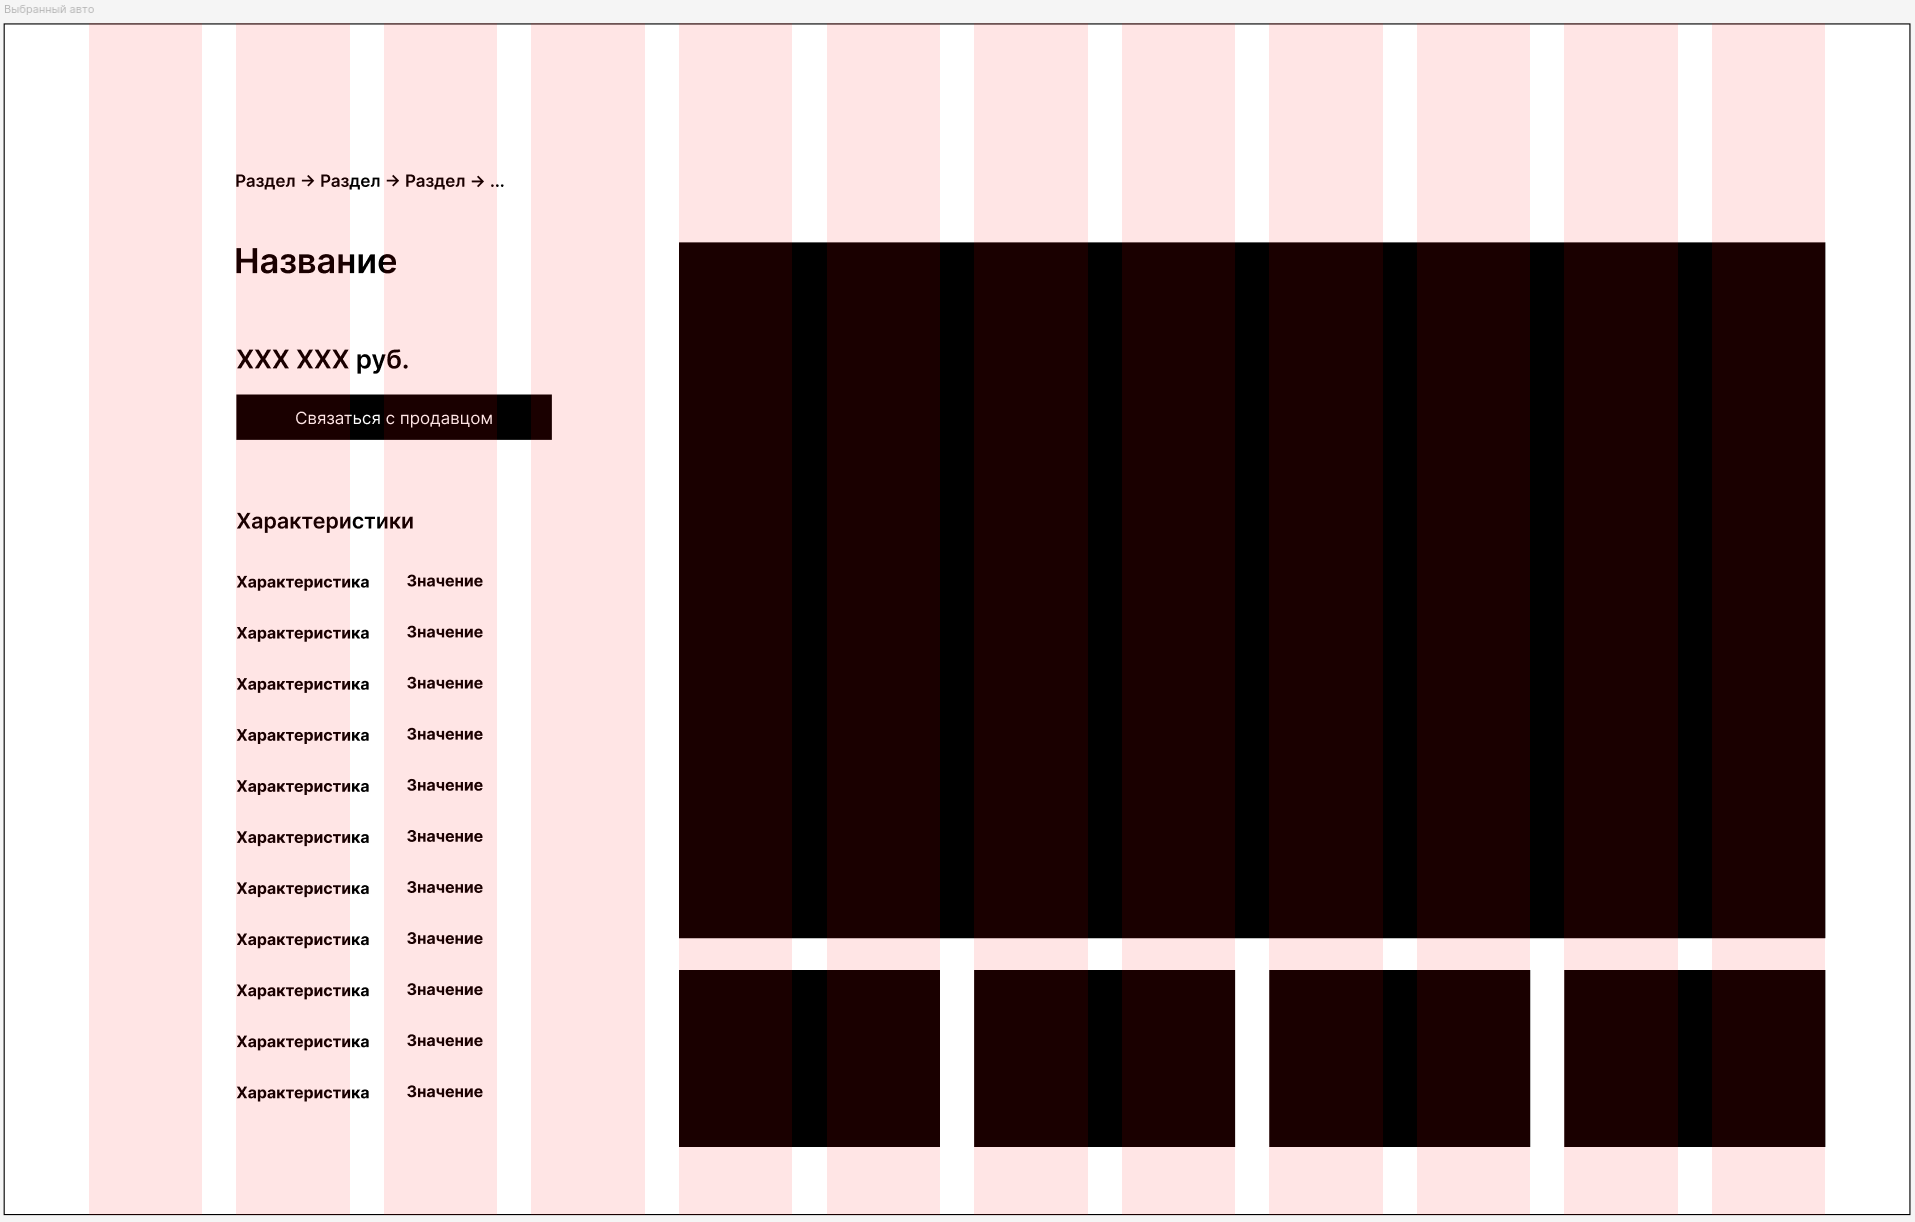
\includegraphics[width=\linewidth]{selected}}
    \captionof{figure}{Выбранный авто}
\end{minipage}
\bigskip

\noindent
\begin{minipage}{\linewidth}
    \fbox{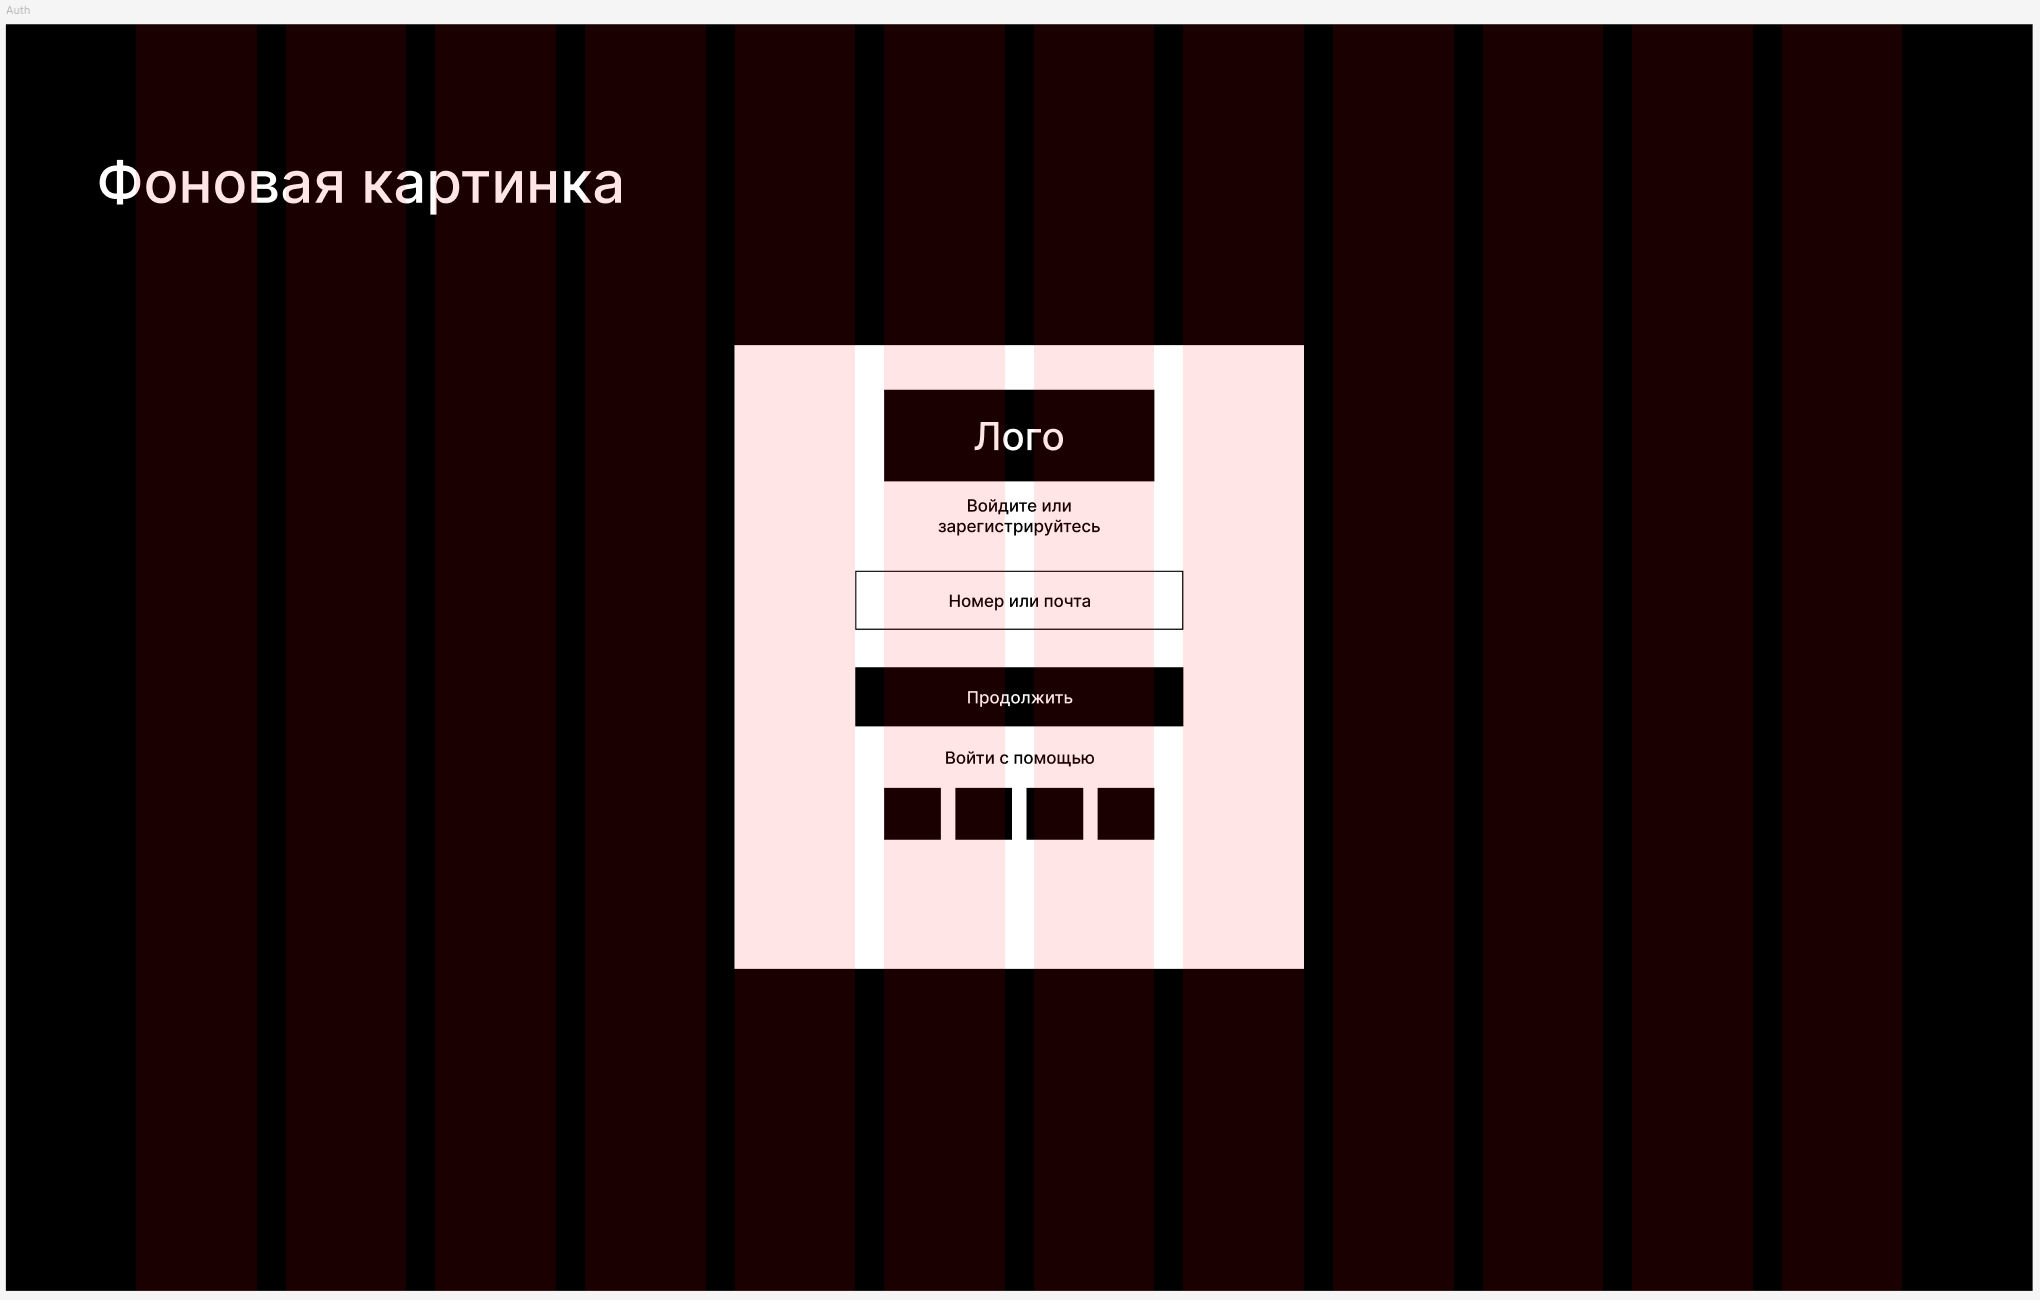
\includegraphics[width=\linewidth]{auth}}
    \captionof{figure}{Авторизация}
\end{minipage}
\bigskip

\noindent
\begin{minipage}{\linewidth}
    \fbox{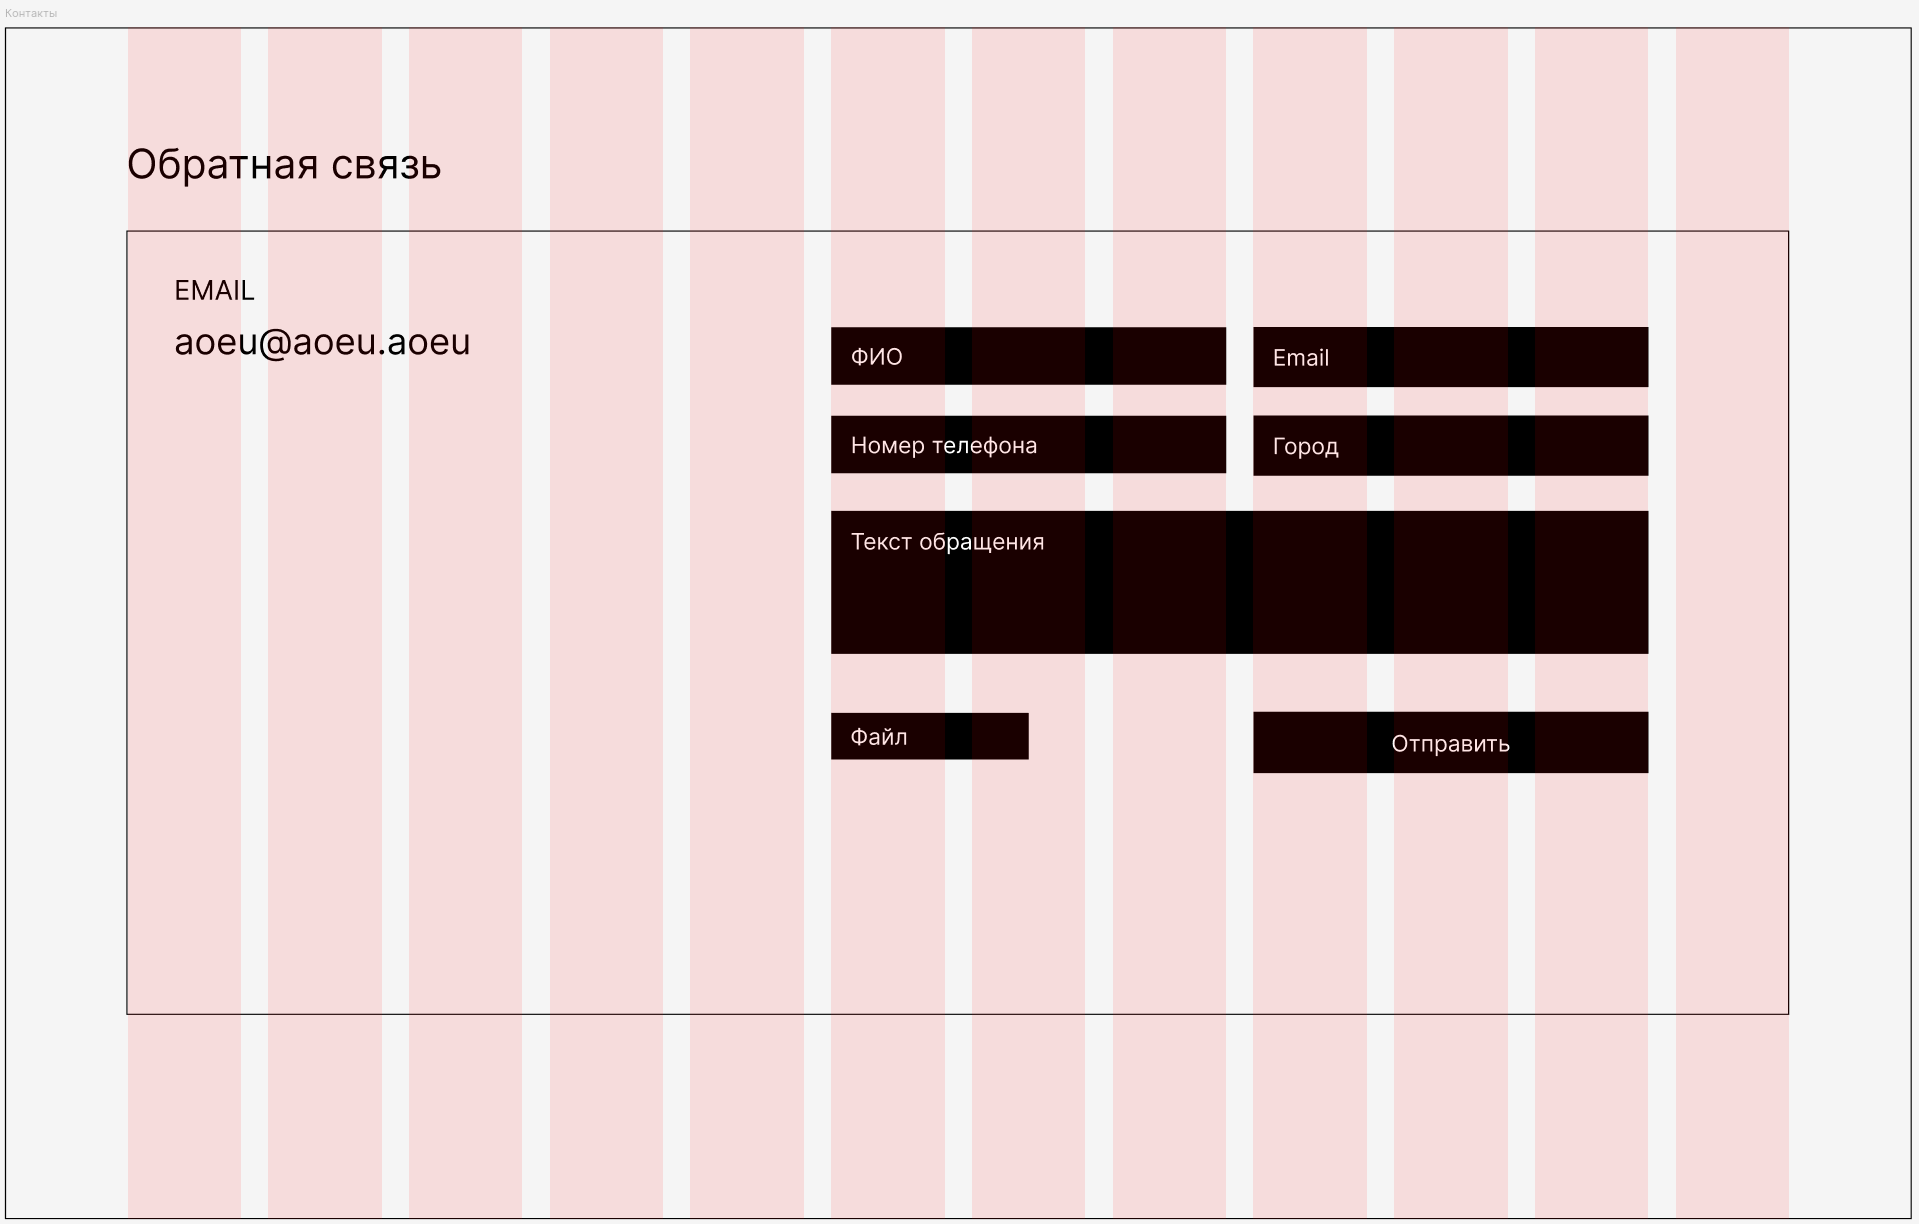
\includegraphics[width=\linewidth]{contacts}}
    \captionof{figure}{Авторизация}
\end{minipage}
\bigskip

\textbf{Контрольные вопросы и ответы}

\begin{enumerate}
    \item Что такое модульная сетка?

Модульная сетка — это структура, основанная на наборе невидимых линий, которая упрощает компоновку элементов на странице и обеспечивает логичность и аккуратность. Она состоит из колонок, межколоночных интервалов и полей, образуя основу для создания организованного интерфейса.

    \item Виды сеток в проектировании

    Одностолбцовая — используется для простых и минималистичных макетов.
    Многостолбцовая — обычно состоит из 12 колонок и применяется для сложных макетов.
    Модульная — сетка, которая объединяет строки и столбцы, создавая сетку ячеек для более гибкой компоновки.
    Иерархическая — используется для макетов с несколькими уровнями структур, где важна иерархия элементов.

    \item Назначение модульной сетки

Модульная сетка помогает упорядочить элементы дизайна, создает визуальный ритм и гармонию, делает интерфейс логичным и удобным. Она также облегчает разработку адаптивных и респонсивных интерфейсов для различных устройств.

    \item Что такое адаптивный дизайн?

Адаптивный дизайн — это подход, при котором разрабатываются несколько фиксированных макетов, каждый из которых оптимизирован для определенного разрешения экрана. При доступе к сайту выбирается наиболее подходящий макет на основе устройства пользователя.

    \item Что такое респонсивный дизайн?

Респонсивный дизайн — это подход, при котором интерфейс динамически подстраивается под размеры экрана благодаря гибким сеткам, изображениями и CSS медиа-запросам, позволяя интерфейсу оставаться удобным на устройствах разного размера.

    \item Назначение респонсивной и адаптивной верстки:

    Адаптивная верстка позволяет создавать макеты, которые более точно подстраиваются под определенные устройства, что дает больший контроль над дизайном на каждом экране.
    Респонсивная верстка обеспечивает плавное изменение макета и упрощает адаптацию интерфейса под любое устройство, обеспечивая универсальный и гибкий подход к отображению контента.
\end{enumerate}

\end{document}
